\subsection{Word segmentation}
\label{sec:segmentation}

Although our CNLM is not equipped with an \emph{a priori} notion of
word, and it is not exposed to the most obvious cue to word boundaries
(whitespace), if it is distilling meaningful linguistic knowledge, we
expect that it should develop some implicit notion of word-like units.
Early work on word segmentation has shown that low transition
probabilities \cite{harris-distributional-1954, saffran-word-1996},
high uncertainty about the next character \cite{cohen-algorithm-2001,
  feng-accessor-2004} and low mutual information
\cite{sun-chinese-1998} serve as statistical cues to word
segmentation.  In Figure~\ref{fig:syntax-depth}, we plot (1) entropy
of the predicted distribution over the next character around word
boundaries, compared to other positions, and (2) the pointwise mutual
information (PMI) between left and right contexts, computed by
subtracting the unconditional likelihood of the next 20 characters
from their likelihood conditioned on the prior context, both computed
using our pre-trained LSTM CNLM on a section of the German training
set.  We see that higher entropy and lower PMI computed on
model-generated probabilities correlate with word boundaries,
suggesting that the model internalized statistics that cue segmentation.

\begin{figure}
	\begin{center}
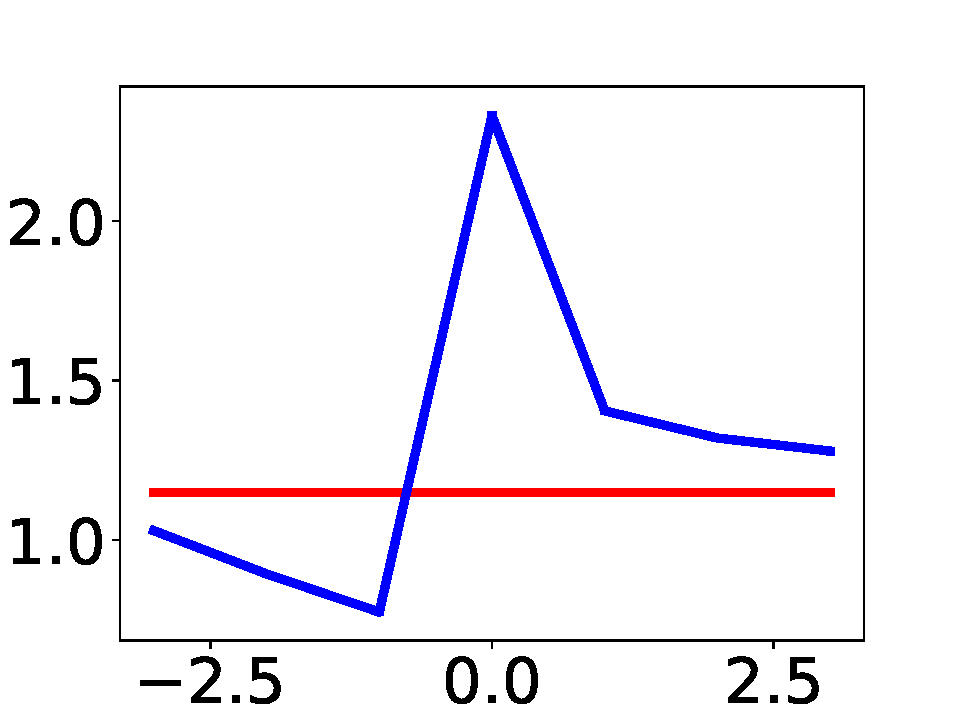
\includegraphics[width=0.22\textwidth]{figures/segmentation-profile-flattened-entropies-english-ci.pdf}
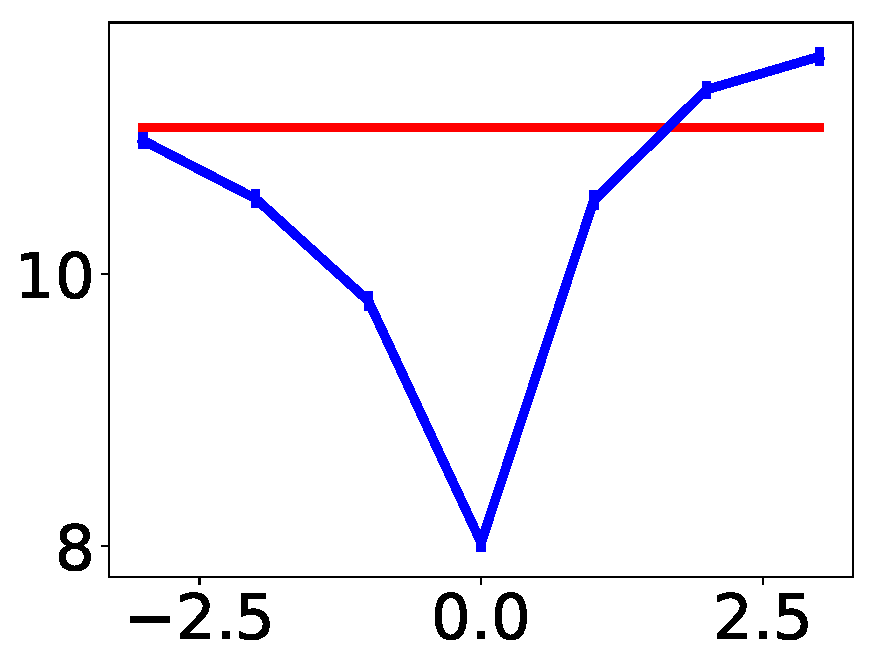
\includegraphics[width=0.22\textwidth]{figures/segmentation-profile-flattened-pmis-english-ci.pdf}
	\end{center}
	\caption{Average entropy over the next character (left) and PMI between left and right contexts (right) around word boundaries (blue); the x-axis indicates position relative to a word boundary. The red line indicates the overall average of the quantity. Error bars indicate (almost imperceptible) bootstrapped 95 \% confidence intervals.}\label{fig:boundaries-entropy}
\end{figure}

To test the model segmentation capabilities more quantitatively, we
used the development sets to train a logistic classifier predicting whether a character is first
in a word or not, based on the following CNLM-derived features: (1)
\emph{surprisal}, the log-probability of the character given prior context, (2)
\emph{entropy} of the distribution over the character given prior
context, (3) \emph{PMI of left and right contexts}, as defined above.
% that is, the total
% likelihood of the next 20 characters, minus the unconditional
% likelihood estimated by starting the CNLM at the current position.
%The rationale of (3) is that it measures the pointwise mutual information, and thus the statistical association, between the subsequent characters and the prior context, which we hypothesize will be higher inside words.
%It is also the transition probability for the next characters
%(3) can also be interpreted as the result of normalizi transition probability
We collected these quantities for each position and for the preceding and following three characters.
%In total, the classifier has 21 coefficients.
We also conducted the same experiment with features extracted from a
character-level 8-gram model estimated on the training set, closer to
the setup of earlier non-neural work. \textbf{Cite some refs here.}


\begin{table*}[t]
  \begin{center}
    \begin{tabular}{l|l|l|l|l}
      \multicolumn{1}{c}{}&\emph{LSTM}&\emph{RNN}&\emph{8-grams}\\
      \hline
      English & 65.8/60.4/63.0 &   63.3/59.8/61.5 & 55.7/51.0/53.3    \\ % \ldots{}/\ldots{}/\ldots & \ldots{}/\ldots{}/\ldots & \ldots{}/\ldots{}/\ldots &\ldots{}/\ldots{}/\ldots\\
      German &  57.0/52.5/54.7 &  53.2/49.3/51.1 & 42.9/36.3/39.3   \\ %   \ldots{}/\ldots{}/\ldots & \ldots{}/\ldots{}/\ldots & \ldots{}/\ldots{}/\ldots &\ldots{}/\ldots{}/\ldots\\
      Italian &  63.6/56.9/60.1 & 62.5/57.5/59.9  & 48.4/39.6/43.6    \\ % \ldots{}/\ldots{}/\ldots & \ldots{}/\ldots{}/\ldots & \ldots{}/\ldots{}/\ldots &\ldots{}/\ldots{}/\ldots\\
    \end{tabular}
  \end{center}
  \caption{\label{tab:segmentation-results} Percentage precision, recall, and F1 on test set word segmentation.}
\end{table*}

%PMI alone 
%P 30.56 R 20.61 F 24.61 German
%P 32.19 R 20.89 F 25.34 Italian
%P 39.37 R 29.45 F 33.69 English
%Surprisal alone
%P 28.04 R 18.64 F 22.4 German
%P 28.76 R 18.31 F 22.38 Italian
%P 33.65 R 24.1 F 28.08 English
%Entropy alone
%P 50.88 R 45.57 F 48.08 German
%P 58.44 R 52.09 F 55.08 Italian
%P 59.85 R 53.75 F 56.63 English


% For each language model and language, we compute how many of the extracted tokens were correct (precision) and how many of the actual tokens were found by the classifier (recall), together with F1.
% The goal of this experiment is not to construct a new word segmentation system, but to evaluate how strongly the CNLM's probabilities are indicative of word boundaries.

Results are shown in Figure~\ref{tab:segmentation-results}. The
CNLM-based classifiers robustly segment more than half of the tokens
correctly, and do considerably better than the character 8-gram model,
with a slight edge for the LSTM. Ablation shows that entropy is most
predictive, reaching an F1 of 56.6\% (English), 48.1\% (German), 55.1\%
(Italian) on its own.%   Surprisal reaches 28.08 (English), 22.4 (German),
% 22.38 (Italian); PMI reaches 33.69 (English), 24.61 (German), 25.34
% (Italian).
%Setting N to other values shows that larger values of N increase performance (N =10: 62.45, N=20: 63.24).

How does the LSTM CNLM compare to \emph{ad-hoc} word segmentation
models?  We compare it to the Bayesian bigram model of
\newcite{goldwater-bayesian-2009}, an elegant model using a
hierarchical Dirichlet process.  The latter, unlike our approach, is
fully unsupervised, but it has a specifically designed built-in bias
towards a discrete lexicon with a power-law frequency distribution.
Moreover, unlike standard supervised word segmentation methods, our
classifier does not have direct access to character strings; instead,
it evaluates how strongly quantities computed by the CNLM
\emph{correlate} with word boundaries. \textbf{Not sure I got the
  latter point.}

Running Bayesian methods on the Wikipedia dumps is computationally
unfeasible. Thus, we re-trained instead the CNLM (with fixed
hyperparameters) on the Brent corpus of child-directed speech
\cite{brent-efficient-1999} also used by Goldwater and colleagues.  We
used 90\% to train our language model, 5\% to fit the logistic
classifier, and 5\% for word segmentation evaluation.  The Bayesian
model is trained and evaluated on the full dataset, as it does not
rely on word boundary information during training. Results in
Table~\ref{tab:segmentation-results-brent} show that the CNLM
performance is broadly comparable to that of a sophisticated Bayesian
segmentation method.

% \begin{table*}[t]
%   \begin{center}
%     \begin{tabular}{ll|l|l|l|l}
%       \multicolumn{2}{c|}{}&Tokens & Lexical & Boundaries\\      \hline
% 	    \multirow{4}{*}{CNLM} & Full model & 0.75/0.76/0.75 & 0.41/0.61/0.49 & 0.91/0.90/0.90 \\
% 	    &     log-probability & 51.0/45.3/48.0 & 48.8/19.5/27.9 & 80.5/71.6/75.8 \\
% 	    &     entropy & 50.4/53.3/51.8 & 52.0/21.1/30.0 & 79.0/74.7/76.8\\
% 	    &     PMI & 70.8/72.9/71.8 & 57.6/34.6/43.2 &89.9/87.3/88.6  \\ \hline
% 	    \multicolumn{2}{c|}{\citet{goldwater-bayesian-2009}} & 75.2/69.6/72.3 & 63.5/55.2/59.1 & 90.3/80.8/85.2
%     \end{tabular}
%   \end{center}
% 	\caption{\label{tab:segmentation-results-brent} Word segmentation results (percentage precision/recall/F1)  on the Brent corpus for our CNLM-based model and the Bayesian approach of \cite{goldwater-bayesian-2009}. Following \cite{goldwater-bayesian-2009}, we evaluate at the level of tokens, the lexicon of induced word types, and boundaries.}
% \end{table*}


\begin{table*}[t]
  \begin{center}
    \begin{tabular}{l|l|l|l|l}
      &Tokens & Lexical & Boundaries\\      \hline
	    CNLM & 75.3/76.6/76.0 & 41.2/61.2/49.2 & 91.3/90.0/90.5 \\
	    \citet{goldwater-bayesian-2009} & 75.2/69.6/72.3 & 63.5/55.2/59.1 & 90.3/80.8/85.2
    \end{tabular}
  \end{center}
	\caption{\label{tab:segmentation-results-brent} Word segmentation results (percentage precision/recall/F1)  on the Brent corpus for our CNLM-based model and the Bayesian approach of \newcite{goldwater-bayesian-2009}. Following them, we evaluate at the level of tokens, the lexicon of induced word types, and boundaries.}
\end{table*}

As a final piece of evidence that the CNLM has internalized a notion
of word, we trained logistic classifiers directly on the hidden states
of the Wikipedia-trained CNLMs. We achieved accuracy above 90\% (and
always above an n-gram-count-based baseline) for all languages, on the
task of classifying word boundaries in unseen words.

%In contrast to the Wikipedia experiments, PMI emerges as the most important predictor on this dataset.

Looking at the main errors made by our English Wikipedia CNLM
segmenter is instructive. We consider first the 30 most common
undersegmentations in the test set (that is, cases in which the model
failed to split two or more words). About half (16) of them are common
function word sequences that could indeed easily be re-analyzed as
single words (e.g., \emph{more than}, \emph{as well as}, \emph{such
  as}). Of the remaining cases, 8 follow the \emph{N of} pattern,
where \emph{N} is a (typically relational) noun commonly occurring in
this construction (\emph{member of}, \emph{end of}, \emph{part
  of}\ldots). There are 3 fixed multi-word expressions (\emph{New
  York}, \emph{United States} and \emph{high school}). Finally, it's
reasonable to treat \emph{based on}, \emph{known as} and
\emph{according to} as lexicalized connectives, especially in the
Wikipedia text the model was trained upon.

The picture is a bit murkier but still fairly linguistically grounded
for the 30 most common oversegmentation errors (that is, the character
fragments that are wrongly segmented from inside the largest number of
distinct words).\footnote{We ignore here single-letter segmentations,
  that would otherwise account for one third of the most-frequent
  set.}  More than half (17) are common affixes (prefixes such as
\emph{re} and \emph{de} or suffixes such as \emph{ing} and
\emph{ly}). The remaining cases include 3 strings identical to frequent
function words wrongly carved out of longer words (\emph{the},
\emph{to} and \emph{on}, although the model might be treating the
latter as a pseudo-suffix in forms such as \emph{Peterson} and
\emph{Creighton}). Further, the strings \emph{land} and \emph{man} are not
unreasonably segmented out of compounds. It's hard, on the other hand,
to find a linguistically sound motivation for the 8 remaining top
oversegmentations (\emph{la, le, ma, na, ra, ro, se, ta}).

To conclude, we reiterate that knowledge about word segmentation is
only implicit in our CNLM, and indeed the same CNLM-generated cues we
relied upon to build our classifier above are actually tracking
boundaries between linguistic constituents of different depth. This is
illustrated by the following test. We created constituency trees for
the German validation set using the Berkeley
Parser~\cite{petrov2007improved}.  For each character in the data, we
counted its hierarchical distance from the preceding character,
operationalized as the number of intervening closing and opening
brackets.  This number is zero if and only if both characters belong
to the same word, 1 at word boundaries. Figure~\ref{fig:syntax-depth}
plots CNLM-based PMI by hierarchical distance, for all distances for
which at least 1,000 data-points occurred in the dataset.  The plot
shows that longer hierarchical distance between neighboring characters
correspond to lower average MI, generalizing the finding for word
boundaries.  This illustrates how it is useful for segmentation
knowledge to be implicit, as the model can discover about different
kinds of boundaries in a continuous manner.

\begin{figure}
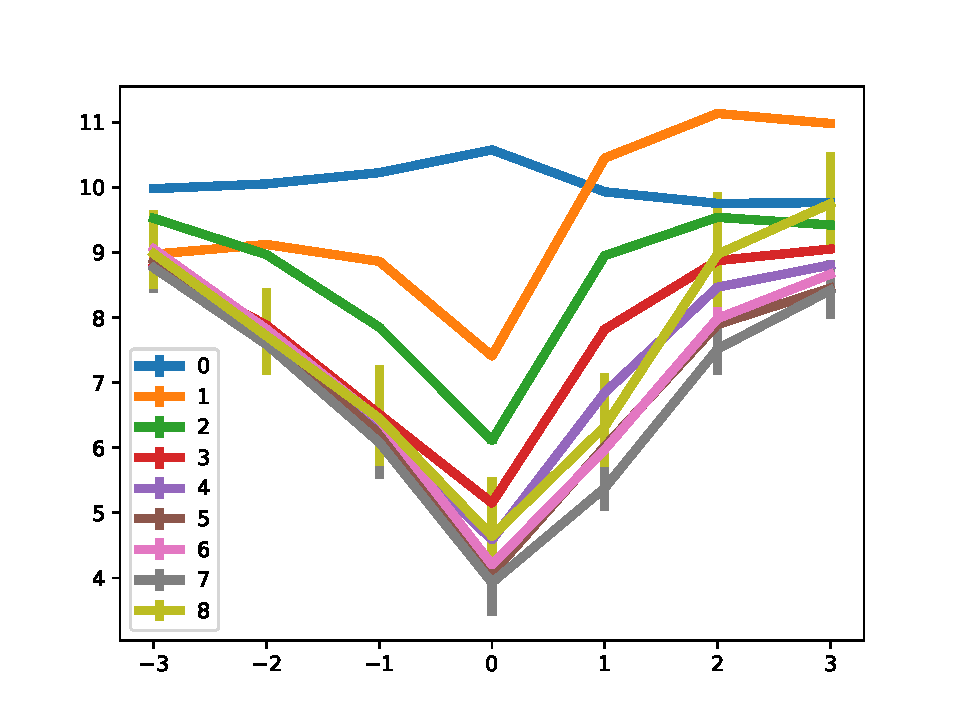
\includegraphics[width=0.48\textwidth]{figures/segmentation-profile-pmis-german-all-heights-ci.pdf}
\caption{PMI between left and right contexts, as estimated by the CNLM in German, organized by syntactic hierarchical distance between subsequent characters (with bootstrapped 95 \% confidence intervals).}\label{fig:syntax-depth}
\end{figure}



%687112
%73757
%46716
%22847
%7896
%2587
%827
%234
%80


